%+++++++++++++++++++++++++++++++++++++++++++++++++++++++++++++++++++++
%Projeto pedagógico do Curso de Engenharia Eletrônica da Universidade Tecnológica Federal do Paraná (UTFPR) - Campus Toledo
%Baseado nas orientações do estilo abntex2 (http://linorg.usp.br/CTAN/macros/latex/contrib/abntex2/doc/abntex2.pdf)
%Autor: Núcleo Docente Estruturante 
% Contato: Prof. Felipe Walter Dafico Pfrimer - pfrimer@utfpr.edu.br
%Ultima atualização: 03/02/2021
%
%+++++++++++++++++++++++++++++++++++++++++++++++++++++++++++++++++++++
%Tipo de documento ABNTEX2:
\documentclass[12pt,openright,oneside,a4paper,
%sumario=tradicional, % para o recomendado pela ABNT utilize sumario=abnt-6027-2012
sumario=abnt-6027-2012,
chapter=TITLE,  % títulos de capítulos convertidos em letras maiúsculas
section=TITLE,  % títulos de seções convertidos em letras maiúsculas
subsection=TITLE, % títulos de subseções convertidos em letras maiúsculas
subsubsection=TITLE, % títulos de subsubseções em letras maiúsculas
subsubsubsection=TITLE, % títulos de subsubsubseções em letras maiúsculas
english,french,spanish,brazil]{abntex2}
%Observe que a ABNT NBR 14724:2011 (seção 5.1) recomenda que os documentos sejam impressos no anverso e no verso das folhas. Isso é obtido com a opção twoside.

%+++++++++++++++++++++++++++++++++++++++++++++++++++++++++++++++++++++
%Pacotes para língua portuguesa do Brasil (código recomendado pelo estilo abntex2):
\usepackage{ifxetex}
\ifxetex
    \usepackage{fontspec}
    \defaultfontfeatures{Ligatures={TeX}}
\else
    \usepackage[utf8]{inputenc}
    \usepackage[T1]{fontenc}
\fi

%Observação: Quando um documento é compilado com xelatex, os pacotes inputenc e fontenc não devem ser incluídos ao preâmbulo do documento. Ao invés desses pacotes, geralmente fontspec é usado. O código anterior de preâmbulo torna flexível a compilação do documento, que pode tanto ser realizada da forma tradicional com pdflatex quanto com xelatex, uma vez que inclui seletivamente os pacotes adequados para cada compilador (página 14 do link http://linorg.usp.br/CTAN/macros/latex/contrib/abntex2/doc/abntex2.pdf).

% Editar o documento "dados_gerais.tex" com as informações do curso
%+++++++++++++++++++++++++++++++++++++++++++++++++++++++++++++++++++++
%Informações do PPC:
\titulo{Projeto Pedagógico do Curso de Engenharia Eletrônica}
\autor{Núcleo Docente Estruturante}
\data{\the\year} % Apenas o ano
\local{Toledo} % Apenas a cidade
\instituicao{Universidade Tecnológica Federal do Paraná
    \par
    Pró-reitoria de graduação e Educação Profissional
    \par
    Campus Toledo}
\tipotrabalho{Projeto Pedagógico do Curso de Engenharia Eletrônica}


%+++++++++++++++++++++++++++++++++++++++++++++++++++++++++++++++++++++
%Preambulo (Texto apresentado na contracapa):

\preambulo{Projeto Pedagógico de Curso apresentado ao Conselho de Graduação e Educação Profissional - COGEP da UTFPR e aprovado pela Resolução \pdfmarkupcomment{COGEP XXX, DE XX/XX/20XX}{Inserir depois de aprovado, ou considerar a primeira aprovação pelo COGEP}}



%+++++++++++++++++++++++++++++++++++++++++++++++++++++++++++++++++++++
%Pacotes adicionais:
\usepackage{amssymb}
\usepackage{tabto}

\usepackage[%
    alf,
    abnt-emphasize=bf,
    bibjustif,
    recuo=0cm,
    abnt-url-package=url,       % Utiliza o pacote url
    abnt-refinfo=yes,           % Utiliza o estilo bibliográfico abnt-refinfo
    abnt-etal-cite=3,
    abnt-etal-list=3,
    abnt-thesis-year=final
]{abntex2cite} 
\usepackage[pdftex]{color,graphicx}
%\usepackage{graphicx}
\usepackage{pdfcomment}
\usepackage{nomencl} % Para a lista abreviaturas e siglas
\makenomenclature    % Para a lista abreviaturas e siglas

% Remove o título original da Nomeclatura:
\renewcommand{\nomname}{}
% Modifica a separação do itens:
\setlength{\nomitemsep}{0pt}
\setlength{\nomlabelwidth}{2.5cm}
% Definição do grupos:
\RequirePackage{ifthen}
 \renewcommand{\nomgroup}[1]{%
     \ifthenelse{\equal{#1}{A}}{\cleardoublepage\item\makebox[0.8\linewidth]{\textbf{\uppercase{\large{Lista de Abreviaturas e Siglas}}}} \makebox[\linewidth]{}\\[0.6cm]}{%
     \ifthenelse{\equal{#1}{S}}{\cleardoublepage\item\makebox[0.8\linewidth]{\textbf{\uppercase{\large{Lista de Símbolos}}}} \makebox[\linewidth]{}\\[0.6cm]}{}}}

\usepackage{indentfirst} % Indenta o primeiro parágrafo de cada seção.
\usepackage{multirow} % Pacote de tabulação para tabelas
\usepackage{bm} % Define o comando \bm para cujo argumento fica em negrito, inclusive formulas matemáticas
\usepackage{lastpage} % Usado por abntex2-fichacatalografica.tex
\usepackage[font=small,labelfont=bf,textfont=bf]{caption} % Legendas de floats em tamanho 10pt e negrito
\usepackage{listings} % Permite digitar códigos em Latex
\usepackage{textcomp} % Pacote com símbolos adicionais para latex (Ex.: baht, bullet, copyright, musicalnote, onequarter, section e yen)
\usepackage{caption} % Permite customizar a legenda de figuras e tabelas
\usepackage{upgreek} % Utilizado para letras gregas não-itálicas
\usepackage{lscape} % Permite rotacionar páginas, mas não os números das páginas.
\usepackage{lipsum} % Para texto filler
\usepackage{verbatim}
\usepackage{listings}
\usepackage{pgfgantt}
\usepackage[a-1b]{pdfx}

\usepackage{hyperref}

%insira novos pacotes aqui:

%+++++++++++++++++++++++++++++++++++++++++++++++++++++++++++++++++++++
%Outras configurações:

% "Por padrão, uma versão sem serifas da fonte corrente do documento é utilizada para os títulos das divisões. Você pode customizar a fonte dos títulos dos capítulos alterando os comandos como no exemplo a seguir, para que seja utilizada a fonte Computer Modern com tamanho maior do que o utilizado por padrão" (manual do abntex2).
\renewcommand{\ABNTEXchapterfont}{\fontfamily{cmr}\fontseries{b}\selectfont}
\renewcommand{\ABNTEXchapterfontsize}{\large}
\renewcommand{\ABNTEXsectionfontsize}{\normalsize}
\renewcommand{\ABNTEXsubsectionfontsize}{\normalsize}
\renewcommand{\ABNTEXsubsubsectionfontsize}{\normalsize}
\renewcommand{\ABNTEXsubsubsubsectionfontsize}{\normalsize}

% Para criação de quadros
% Novo list of (listings) para QUADROS:
\newcommand{\quadroname}{Quadro}
\newcommand{\listofquadrosname}{Lista de quadros}

\newfloat[chapter]{quadro}{loq}{\quadroname}
\newlistof{listofquadros}{loq}{\listofquadrosname}
\newlistentry{quadro}{loq}{0}

% configurações para atender às regras da ABNT (não remover ou alterar) 
\setfloatadjustment{quadro}{\centering}
\counterwithout{quadro}{chapter}
\renewcommand{\cftquadroname}{\quadroname\space} 
\renewcommand*{\cftquadroaftersnum}{\hfill--\hfill}

% Configuração de posicionamento padrão:
\setfloatlocations{quadro}{hbtp}


%\setlength\afterchapskip{\lineskip} % Espaçamento de 1,5 entre o título do capítulo e corpo do texto

% informações do PDF
\makeatletter
\hypersetup{
	%pagebackref=true,
	pdftitle={Teste}, 
	pdfauthor={\imprimirautor},
	pdfsubject={\imprimirpreambulo},
	pdfcreator={LaTeX with abnTeX2},
	pdfkeywords={abnt}{latex}{abntex}{abntex2}{livro}, 
	colorlinks=true,       		% false: boxed links; true: colored links
	linkcolor=blue,          	% color of internal links
	citecolor=blue,        		% color of links to bibliography
	filecolor=magenta,      		% color of file links
	urlcolor=blue,
	bookmarksdepth=4
}
\makeatother
% ---
\makeatletter
\pdfinfo {   
	/Title (teste)
	/Author (teste)
	/Subject (teste)
	/Keywords (teste) 
}
\makeatother

%+++++++++++++++++++++++++++++++++++++++++++++++++++++++++++++++++++++
%Início do documento:
\begin{document}
    %+++++++++++++++++++++++++++++++++++++++++++++++++++++++++++++++++
    % Elementos pré-textuais
    \pretextual

    % Imprime capa e pula sua numeração
    \pagenumbering{gobble} % Remove a visualização da numeração das páginas e reinicia em 1 
    \clearpage
    \thispagestyle{empty}
    \imprimircapa
    \clearpage
    \pagenumbering{arabic}% Numeração arábica (e reinicia em 1)

    % Imprime a folha de rosto (padrão do abntex2)
    \imprimirfolhaderosto*

    % Insere a ficha catalográfica (Não utilizado pela UTFPR até o momento, manter comentado)
    %\begin{fichacatalografica}
    \sffamily
    \vspace*{15cm}    % Posição vertical
    \hrule       % Linha horizontal
    \begin{center}    % Minipage Centralizado
        \begin{minipage}[c]{12.5cm} % Largura
            \imprimirautor
            \hspace{0.5cm} \imprimirtitulo / \imprimirautor. --
            \imprimirlocal, \imprimirdata-
            \hspace{0.5cm} \pageref{LastPage} p. : il.(alguma color.); 30 cm.\\
            \hspace{0.5cm} \imprimirorientadorRotulo \imprimirorientador\\
            \hspace{0.5cm}
            \parbox[t]{\textwidth}{\imprimirtipotrabalho~--~\imprimirinstituicao,
            \imprimirdata.}\\
            \hspace{0.5cm}
            1. Palavra-chave1.
            2. Palavra-chave2.
            I. Orientador.
            II. Universidade xxx.
            III. Faculdade de xxx.
            IV. Título\\
            \hspace{8.75cm} CDU 02:141:005.7\\
        \end{minipage}
    \end{center}
\hrule
\end{fichacatalografica}

    % Insere a folha de aprovação (Obrigatório para TCC2)
    %\begin{folhadeaprovacao}
    \begin{center}
        {\ABNTEXchapterfont\large\imprimirautor}
        \vspace*{\fill}\vspace*{\fill}
            \begin{center}
                \ABNTEXchapterfont\bfseries\Large\imprimirtitulo
            \end{center}
            \vspace*{\fill}
            \hspace{.45\textwidth}
            \begin{minipage}{.5\textwidth}
                \imprimirpreambulo
            \end{minipage}%
            \vspace*{\fill}
    \end{center}
    Trabalho aprovado. \imprimirlocal, 24 de novembro de 2012:
    
    % Editar as próximas três linhas:
    \assinatura{\textbf{\imprimirorientador} \\ Nome do Orientador}
    \assinatura{\textbf{Professor} \\ Nome do Convidado 1}
    \assinatura{\textbf{Professor} \\ Nome do Convidado 2}
    
    \begin{center}
        \vspace*{0.5cm}
        {\large\imprimirlocal}
        \par
        {\large\imprimirdata}
        \vspace*{1cm}
    \end{center}
\end{folhadeaprovacao} % Altere o arquivo folha-de-aprovacao.tex com as informações do seu TCC
    
    % Insere o resumo e o abstract (Obrigatório para TCC2)
    \clearpage\mbox{}\clearpage

% --- resumo em português --- (Obrigatório para TCC2)
\begin{resumo}
    Resumo aqui.
    
    \vspace{\onelineskip}
    \noindent
    \textbf{Palavras-chave}: Palavra 1. Palavra 2. Palavra 3. % inserir até cinco palavras
\end{resumo}

% --- resumo em inglês --- (Obrigatório para TCC2)
% \begin{resumo}[Abstract]
%     \begin{otherlanguage*}{english}
%         Abstract here.
        
%         \vspace{\onelineskip}
%         \noindent
%         \textbf{Keywords}: Palavra 1. Palavra 2. Palavra 3. % inserir até cinco palavras
%     \end{otherlanguage*}
% \end{resumo}


 %resumo (deve conter resumo)

    %Lista de figuras
    \pdfbookmark[0]{\listfigurename}{lof}
    \listoffigures* 
    \cleardoublepage

    %Lista de tabelas (Opcional)
    %\listoftables

    %lista de abreviaturas e siglas
    \pdfbookmark[0]{\nomname}{lst}
    \printnomenclature
    \cleardoublepage

    %Sumário
    \pdfbookmark[0]{\contentsname}{toc}
    \tableofcontents*
    \cleardoublepage
    
    %+++++++++++++++++++++++++++++++++++++++++++++++++++++++++++++++++
    % Elementos textuais
    \textual
    
    % A estrutura deve respeitar as normas da ABNT
    \chapter{CAPÍTULO, NÍVEL 1}
\label{chap:nivel1}

    Toda seção deve conter um corpo de texto, obrigatoriamente. Insira um novo capítulo com o comando \verb|\chapter{<título>}|, substituindo \verb|<título>| pelo título do capítulo. Use o comando \verb|label{<chave>}| logo após \verb|\chapter{}| para utilizar referência cruzada. O \autoref{qua:intro} mostra um exemplo de código. Observação: se utilizar o sumário tradicional (veja a declaração \verb|\documentclass[]{}| no arquivo \verb|main.tex|) escreva o título capitalizado para garantir que os títulos fiquem em maiúsculo no sumário. Essa observação também é válida para seções e subseções.
    
\begin{quadro}[!htb]
    \centering
    \caption{Exemplo de novo capítulo \label{qua:intro}}
    \begin{tabular}{|c|l|}
        \hline
        1 &\verb|\chapter{Introdução}|\\
        2 &\verb|\label{chap:intro}|\\
        3 &\\
        4 &\verb|<texto>|\\
        \hline
    \end{tabular}
    \fonte{Autoria própria}
\end{quadro}

\nomenclature[S]{$T_S$}{Temperatura}
\nomenclature[S]{$X_i$}{Ponto inicial}

\section{SEÇÃO, NÍVEL 2}
\label{sec:nivel2}

    Essa é uma seção, nível 2, do \autoref{chap:nivel1}. Utilize o comando \verb|\section{<título>}| para criar uma nova seção de nível 2. O \autoref{qua:sec} mostra um exemplo de código.
    
    \begin{quadro}[!htb]
    \centering
    \caption{Exemplo de nova seção de nível 2 \label{qua:sec}}
    \begin{tabular}{|c|l|}
        \hline
        1 &\verb|\section{A vida da marmota}|\\
        2 &\verb|\label{sec:marm}|\\
        3 &\\
        4 &\verb|<texto>|\\
        \hline
    \end{tabular}
    \fonte{Autoria própria}
    \end{quadro}
    
\subsection{SUBSEÇÃO, NÍVEL 3}
\label{subsec:nivel3}

    Essa é uma subseção, nível 3, da \autoref{sec:nivel2}. Caso seja necessário criar uma seção desse tipo em seu texto, utilize o comando \verb|\subsection{<título>}| para criar uma nova seção de nível 3. O \autoref{qua:subsec} mostra um exemplo de código.
    
    \begin{quadro}[!htb]
    \centering
    \caption{Exemplo de nova seção de nível 3 \label{qua:subsec}}
    \begin{tabular}{|c|l|}
        \hline
        1 &\verb|\subsection{Onde vivem}|\\
        2 &\verb|\label{sec:viva}|\\
        3 &\\
        4 &\verb|<texto>|\\
        \hline
    \end{tabular}
    \fonte{Autoria própria}
    \end{quadro}
    
\subsubsection{SUBSEÇÃO, NÍVEL 4}
\label{subsubsec:nivel4}

    Essa é uma subseção, nível 4, da \autoref{subsec:nivel3}. Caso seja necessário criar uma seção desse tipo em seu texto, utilize o comando \verb|\subsubsection{<título>}| para criar uma nova seção de nível 4. O \autoref{qua:subsubsec} mostra um exemplo de código.
    
    \begin{quadro}[!htb]
    \centering
    \caption{Exemplo de nova seção de nível 4 \label{qua:subsubsec}}
    \begin{tabular}{|c|l|}
        \hline
        1 &\verb|\subsubsection{O que comem}|\\
        2 &\verb|\label{sec:food}|\\
        3 &\\
        4 &\verb|<texto>|\\
        \hline
    \end{tabular}
    \fonte{Autoria própria}
    \end{quadro}
    
\subsubsubsection{SUBSEÇÃO, NÍVEL 5}
\label{subsubsubsec:nivel5}

    Isso é uma subseção, nível 5, da \autoref{subsubsec:nivel4}. Pela norma da Associação Brasileira de Normas Técnicas (ABNT), \nomenclature[A]{ABNT}{Associação Brasileira de Normas Técnicas} subseções são permitidas até o nível 5 \cite{NBR6024:2012}. Caso seja necessário criar uma seção desse tipo em seu texto, utilize o comando \verb|\subsubsubsection{<título>}| para criar uma nova seção de nível 5. O \autoref{qua:subsubsubsec} mostra um exemplo de código.
    
    \begin{quadro}[!htb]
    \centering
    \caption{Exemplo de nova seção de nível 5 \label{qua:subsubsubsec}}
    \begin{tabular}{|c|l|}
        \hline
        1 &\verb|\subsubsubsection{Como se reproduzem}|\\
        2 &\verb|\label{sec:sex}|\\
        3 &\\
        4 &\verb|<texto>|\\
        \hline
    \end{tabular}
    \fonte{Autoria própria}
    \end{quadro}
    
\section{SIGLAS, ACRÔNIMOS E SÍMBOLOS}
\label{sec:siglas}

    Para acrescentar uma sigla ou acrônimo na lista de siglas e acrônimos utilize o comando \verb|\nomenclature[A]{<sigla>}{<significado>}| em qualquer parte do texto. É recomendado inserir esse comando logo após a primeira aparição da sigla ou do acrônimo. Um exemplo de código está transcrito no \autoref{qua:siglacode}. 
    
    \begin{quadro}[!htb]
    \centering
    \caption{Exemplo de código para a acrescentar siglas ou acrônimos na lista \label{qua:siglacode}}
    \begin{tabular}{|l|}
        \hline
        \makebox[0.9\linewidth]{\textbf{Código}}\\
        \hline
        \verb|A Ordem dos Advogados do Brasil (OAB) \nomenclature[A]{OAB}{Ordem dos|\\
        \verb|Advogados do Brasil} diz que apoia investigação do ataque de milícias|\\
        \verb|digitais ao Supremo Tribunal Federal (STF) \nomenclature[A]{STF}|\\
        \verb|{Supemo Tribunal Federal}.|\\
        \hline
        \hline
        \makebox[0.9\linewidth]{\textbf{Resultado}}\\
        \hline
        A Ordem dos Advogados do Brasil (OAB) \nomenclature[A]{OAB}{Ordem dos|Advogados do Brasil} diz que apoia investigação do ataque de \\
        milícias digitais ao Supremo Tribunal Federal (STF) \nomenclature[A]{STF}{Supemo Tribunal Federal}.\\
        \hline
    \end{tabular}
    \fonte{Autoria própria}
    \end{quadro}
    
    
    
    
    Para acrescentar um símbolo na lista de símbolos utilize o comando \verb|\nomenclature[S]| \verb|{<simbolo>}{<significado>}| em qualquer parte do texto. É recomendado inserir esse comando logo após a primeira aparição do símbolo. Um exemplo de código está transcrito no \autoref{qua:simbcode}.
    
    \begin{quadro}[!htb]
    \centering
    \caption{Exemplo de código para a acrescentar símbolos na lista \label{qua:simbcode}}
    \begin{tabular}{|l|}
        \hline
        \makebox[0.9\linewidth]{\textbf{Código}}\\
        \hline
        \verb|A segunda lei de Newton diz que $F_r = ma$, onde $F_r$|\\
        \verb|\nomenclature[S]{$F_r$}{Força resultante} é a força resultante, $m$|\\
        \verb|\nomenclature[S]{$m$}{massa} é a massa e $a$ \nomenclature[S]{$a$}|\\
        \verb|{aceleração} é a aceleração.|\\
        \hline
        \hline
        \makebox[0.9\linewidth]{\textbf{Resultado}}\\
        \hline
        A segunda lei de Newton diz que $F_r = ma$, onde $F_r$ \nomenclature[S]{$F_r$}{Força resultante} é a força resultante,\\
        $m$ \nomenclature[S]{$m$}{massa} é a massa e $a$ \nomenclature[S]{$a$}{aceleração} é a aceleração.\\
        \hline
    \end{tabular}
    \fonte{Autoria própria}
    \end{quadro}
    
    Para que as listas sejam geradas é necessário que o comando \textit{\textbf{makeindex}} seja executado com os seguintes argumentos: 
    
    \makebox[0.95\linewidth]{makeindex -s nomencl.ist -o main.nls main.nlo}
    
    \noindent onde ``main'' é o nome do arquivo principal do projeto. Procure mais informações na base de dados do seu editor e copilador \LaTeX.
    
    
\section{SOBRE AS REFERÊNCIAS CRUZADAS E ITENS NUMERADOS}
\label{sec:refs}

    A numeração sequencial de figuras, tabelas, quadros e equações ocorre de modo automático. As ilustrações (figuras), tabelas e quadros serão indexadas automaticamente em suas respectivas listas. 

    Referências cruzadas são obtidas através dos comandos \verb|\label{}| e \verb|\ref{}|. Sendo assim, não é necessário por exemplo, saber que o número de certo capítulo para colocar o seu número no texto. O comando \verb|\autoref{}| facilita referenciação de elementos numerados no texto sem a necessidade de nomear o tipo do elemento.
    
    Observe que este capítulo recebeu a chave ``chap:nivel1'' através do comando \verb|\label{}| (\verb|\label{chap:nivel1}|). Dessa forma, ao utilizar o código \verb|\ref{chap:nivel1}| resulta na escrita do número do capítulo que nesse caso é ``\ref{chap:nivel1}''. De forma análoga, o comando \verb|\autoref{chap:nivel1}| resulta em ``\autoref{chap:nivel1}''.
    
\section{FIGURAS}
\label{sec:figuras}

    Esta seção trata de um exemplo de como inserir uma figura. Note que a \autoref{fig:figura-exemplo1} aparece automaticamente na lista de figuras. Para saber mais sobre o uso de imagens no \LaTeX{} consulte literatura especializada \cite{Goossens2007}.

    \begin{figure}[!htb]
        \centering
        \caption{Exemplo de Figura}
        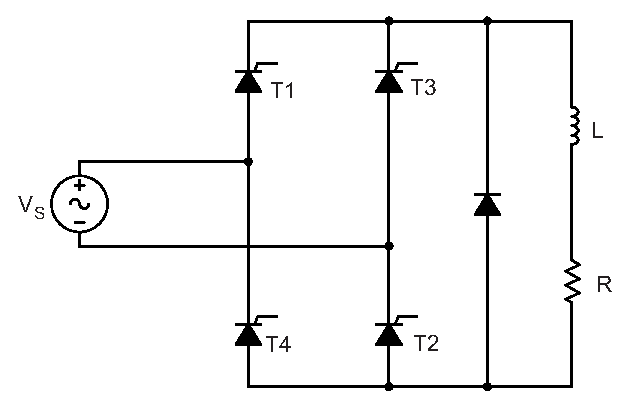
\includegraphics[width=0.6\textwidth]{Caps/Figs/exemplo.eps}
        \fonte{Autoria Própria}
        \label{fig:figura-exemplo1}
    \end{figure}
    
    O código utilizado para inserir a \autoref{fig:figura-exemplo1} está listado no \autoref{qua:figura}.
    
    \begin{quadro}[!htb]
    \centering
    \caption{Código exemplo utilizado para inserir a \autoref{fig:figura-exemplo1} \label{qua:figura}}
    \begin{tabular}{|c|l|}
        \hline
        1 &\verb|\begin{figure}[!htb]|\\
        2 &\verb|\centering|\\
        3 &\verb|\caption{Exemplo de Figura}|\\
        4 &\verb|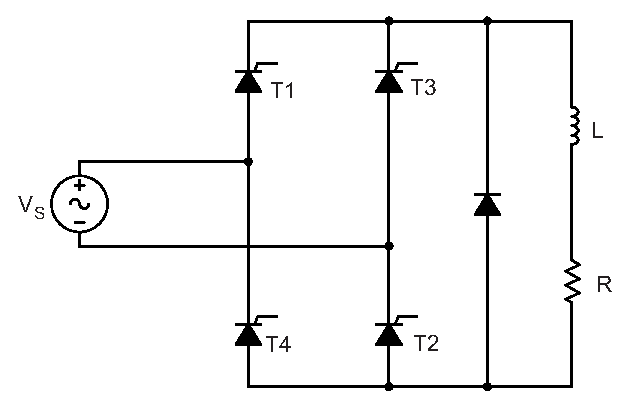
\includegraphics[width=0.6\textwidth]{Caps/Figs/exemplo.eps}|\\
        5 &\verb|\fonte{Autoria Própria}|\\ 
        6 &\verb|\label{fig:figura-exemplo1}|\\ 
        7 &\verb|\end{figure}|\\ 
        \hline
    \end{tabular}
    \fonte{Autoria própria}
    \end{quadro}
    
    Utilize figuras no formato \textit{Encapsulated PostScript} (EPS)\nomenclature[A]{EPS}{\textit{Encapsulated PostScript}}. Caso precise de outro formato, acrescente no preambulo deste modelo o pacote adequado para a sua necessidade.
    
\section{QUADROS E TABELAS}
\label{sec:tabelas}

    Esta seção trata de exemplos de como inserir o \autoref{qua:quadro-exemplo1} e a \autoref{tab:tabela-exemplo1}. Ambos aparecem automaticamente nas suas respectivas listas. Para saber mais informações sobre a construção de tabelas no \LaTeX{} consulte literatura especializada \cite{Mittelbach2004}.

    \begin{quadro}[!htb]
    \centering
    \caption{Exemplo de Quadro \label{qua:quadro-exemplo1}}
    \begin{tabular}{|p{7cm}|p{7cm}|}
        \hline
        \textbf{BD Relacionais} & \textbf{BD Orientados a Objetos} \\
        \hline
        Os dados são passivos, ou seja, certas operações limitadas podem ser automaticamente acionadas quando os dados são usados. Os dados são ativos, ou seja, as solicitações fazem com que os objetos executem seus métodos. & Os processos que usam dados mudam constantemente. \\
        \hline
    \end{tabular}
    \fonte{\citeonline{Barbosa2004}}
    \end{quadro}

    A diferença entre quadro e tabela está no fato que um quadro é formado por linhas horizontais e verticais. Deve ser utilizado quando o conteúdo é majoritariamente não-numérico. O número do quadro e o título vem acima do quadro, e a fonte, deve vir abaixo. Uma tabela é formada apenas por linhas verticais. Deve ser utilizada quando o conteúdo é majoritariamente numérico. O número da tabela e o título vem acima da tabela, e a fonte, deve vir abaixo, tal como no quadro.

    \begin{table}[!htb]
    \centering
    \caption[Resultado dos testes]{Resultado dos testes
    \label{tab:tabela-exemplo1}}
    \begin{tabular}{rrrrr}
        \toprule
            & Valores 1 & Valores 2 & Valores 3 & Valores 4 \\
        \midrule
            Caso 1 & 0,86 & 0,77 & 0,81 & 163 \\
            Caso 2 & 0,19 & 0,74 & 0,25 & 180 \\
            Caso 3 & 1,00 & 1,00 & 1,00 & 170 \\
        \bottomrule
    \end{tabular}
    \fonte{\citeonline{Barbosa2004}}
    \end{table}
    
    Os códigos para inserção do \autoref{qua:quadro-exemplo1} e da \autoref{tab:tabela-exemplo1} estão disponíveis nos Quadros \ref{qua:quaex} e \ref{qua:tabex}.
    
    \begin{quadro}[!htb]
    \centering
    \caption{Código exemplo utilizado para inserir o \autoref{qua:quadro-exemplo1} \label{qua:quaex}}
    \begin{tabular}{|p{0.9\linewidth}|}
    \hline
    \begin{verbatim}
\begin{quadro}[!htb]
\centering
\caption{Exemplo de Quadro \label{qua:quadro-exemplo1}}
    \begin{tabular}{|p{7cm}|p{7cm}|}
    \hline
    \textbf{BD Relacionais} & \textbf{BD Orientados a Objetos} \\
    \hline
    Os dados são passivos, ou seja, certas operações limitadas 
    podem ser automaticamente acionadas quando os dados são 
    usados. Os dados são ativos, ou seja, as solicitações fazem 
    com que os objetos executem seus métodos. & Os processos 
    que usam dados mudam constantemente. \\
    \hline
    \end{tabular}
\fonte{\citeonline{Barbosa2004}}
\end{quadro}
    \end{verbatim}
    \\
    \hline
    \end{tabular}
    \fonte{Autoria própria}
    \end{quadro}
    
    \begin{quadro}[!htb]
    \centering
    \caption{Código exemplo utilizado para inserir a \autoref{tab:tabela-exemplo1} \label{qua:tabex}}
    \begin{tabular}{|p{0.9\linewidth}|}
    \hline
    \begin{verbatim}
\begin{table}[!htb]
\centering
\caption[Resultado dos testes]{Resultado dos testes
\label{tab:tabela-exemplo1}}
    \begin{tabular}{rrrrr}
        \toprule
            & Valores 1 & Valores 2 & Valores 3 & Valores 4 \\
        \midrule
            Caso 1 & 0,86 & 0,77 & 0,81 & 163 \\
            Caso 2 & 0,19 & 0,74 & 0,25 & 180 \\
            Caso 3 & 1,00 & 1,00 & 1,00 & 170 \\
        \bottomrule
    \end{tabular}
\fonte{\citeonline{Barbosa2004}}
\end{table}
    \end{verbatim}
    \\
    \hline
    \end{tabular}
    \fonte{Autoria própria}
    \end{quadro}
    
\section{EQUAÇÕES}
\label{sec:equacoes}

    Esta seção trata de exemplos de como inserir a Eq. (\ref{eq:equacao-exemplo1}) e a Eq. (\ref{eq:equacao-exemplo2}) no corpo do texto \footnote{Deve-se atentar ao fato de a formatação das equações ficar muito boa esteticamente.}. Observe que foram utilizadas duas formas distintas para referenciar as equações. Os códigos utilizados estão no \autoref{qua:eqex}.

    \begin{equation}
        X(s) = \int\limits_{t = -\infty}^{\infty} x(t)  \mathrm{e}^{-st}  dt
        \label{eq:equacao-exemplo1}
    \end{equation}

    \begin{equation}
        F(u, v) = \sum_{m = 0}^{M - 1} \sum_{n = 0}^{N - 1} f(m, n) \exp \left[ -j 2 \pi \left( \frac{u m}{M} + \frac{v n}{N} \right) \right]
        \label{eq:equacao-exemplo2}
    \end{equation}
    
    \begin{quadro}[!htb]
    \centering
    \caption{Código exemplo utilizado para inserir as Equações (\ref{eq:equacao-exemplo1}) e (\ref{eq:equacao-exemplo2}) \label{qua:eqex}}
    \begin{tabular}{|p{0.9\linewidth}|}
    \hline
    \begin{verbatim}
\begin{equation}
    X(s) = \int\limits_{t = -\infty}^{\infty} x(t)\text{e}^{-st}dt
    \label{eq:equacao-exemplo1}
\end{equation}

\begin{equation}
    F(u, v) = \sum_{m = 0}^{M - 1} \sum_{n = 0}^{N - 1} f(m, n) 
    \exp \left[ -j 2 \pi \left( \frac{u m}{M} + \frac{v n}{N} 
    \right) \right]
    \label{eq:equacao-exemplo2}
\end{equation}
    \end{verbatim}
    \\
    \hline
    \end{tabular}
    \fonte{Autoria própria}
    \end{quadro}
    
\section{SOBRE AS LISTAS}
\label{sec:apSobreLista}

    Exemplo de duas listas não numeradas aninhadas, utilizando o comando \verb|\itemize|. Observe a indentação, bem como a mudança automática do tipo de "\textit{bullet}"{} nas listas aninhadas.

    \begin{itemize}
        \item item não numerado 1
        \item item não numerado 2
        \begin{itemize}
            \item subitem não numerado 1
            \item subitem não numerado 2
            \item subitem não numerado 3
        \end{itemize}
        \item item não numerado 3
    \end{itemize}

    Exemplo de duas listas numeradas aninhadas, utilizando o comando \verb|\enumerate|. Observe a numeração progressiva e indentação das listas aninhadas.

    \begin{enumerate}
        \item item numerado 1
        \item item numerado 2
        \begin{enumerate}
            \item subitem numerado 1
            \item subitem numerado 2
            \item subitem numerado 3
        \end{enumerate}
        \item item numerado 3
    \end{enumerate}
    
\subsection{CITAÇÕES INDIRETAS}
\label{subsec:citacoesLivres}

    É a transcrição, com suas próprias palavras, das idéias de um autor, mantendo-se o sentido original. A citação indireta é a maneira que o pesquisador tem de ler, compreender e gerar conhecimento a partir do conhecimento de outros autores. Quanto à chamada da referência, ela pode ser feita de duas maneiras distintas, conforme o nome do(s) autor(es) façam parte do seu texto ou não. Exemplo de chamada fazendo parte do texto:
    
    \vspace{1cm}
    
    Enquanto \citeonline{Maturana2003} defendem uma epistemologia baseada na biologia. Para os autores, é necessário rever \ldots
    
    \vspace{1cm}

    A chamada de referência foi feita com o comando \verb|\citeonline{chave}|, que produzirá a formatação correta.

    A segunda forma de fazer uma chamada de referência deve ser utilizada quando se quer evitar uma interrupção na sequência do texto, o que poderia, eventualmente, prejudicar a leitura. Assim, a citação é feita e imediatamente após a obra referenciada deve ser colocada entre parênteses. Porém, neste caso específico, o nome do autor deve vir em caixa alta, seguido do ano da publicação. Exemplo de chamada não fazendo parte do texto:
    
    \vspace{1cm}
    
    Há defensores da epistemologia baseada na biologia que argumentam em favor da necessidade de \ldots \cite{Maturana2003}.
    
    \vspace{1cm}
    
    Nesse caso a chamada de referência deve ser feita com o comando \verb|\cite{chave}|, que produzirá a formatação correta.
    
\subsection{CITAÇÕES DIRETAS}
\label{subsec:citacoesLiterais}

    É a transcrição ou cópia de um parágrafo, de uma frase, de parte dela ou de uma expressão, usando exatamente as mesmas palavras adotadas pelo autor do trabalho consultado.

    Quanto à chamada da referência, ela pode ser feita de qualquer das duas maneiras já mencionadas nas citações indiretas, conforme o nome do(s) autor(es) façam parte do texto ou não. Há duas maneiras distintas de se fazer uma citação direta, conforme o trecho citado seja longo ou curto.

    Quando o trecho citado é longo (4 ou mais linhas) deve-se usar um parágrafo específico para a citação, na forma de um texto recuado (4 cm da margem esquerda), com tamanho de letra menor e espaçamento entrelinhas simples. Exemplo de citação longa:
    
    \vspace{1cm}
    
    \begin{citacao}
        Desse modo, opera-se uma ruptura decisiva entre a reflexividade filosófica, isto é a possibilidade do sujeito de pensar e de refletir, e a objetividade científica. Encontramo-nos num ponto em que o conhecimento científico está sem consciência. Sem consciência moral, sem consciência reflexiva e também subjetiva. Cada vez mais o desenvolvimento extraordinário do conhecimento científico vai tornar menos praticável a própria possibilidade de reflexão do sujeito sobre a sua pesquisa \cite[p.~28]{Silva2000}.
    \end{citacao}

    Para fazer a citação longa deve-se utilizar os seguintes comandos:
    \begin{verbatim}
\begin{citacao}
<texto da citacao>
\end{citacao}
    \end{verbatim}

    No exemplo, para a chamada da referência o comando \verb|\cite[p.~28]{Silva2000}| foi utilizado, visto que os nomes dos autores não são parte do trecho citado. É necessário também indicar o número da página da obra citada que contém o trecho citado.

    Quando o trecho citado é curto (3 ou menos linhas) ele deve inserido diretamente no texto entre aspas. Exemplos de citação curta:
    
    \vspace{1cm}
    
    A epistemologia parte do princípio de que "assumo que não posso fazer referência a entidades independentes de mim para construir meu explicar" \cite[p.~35]{Maturana2003}.
    
    \vspace{1cm}
    
    A epistemologia baseada na biologia de \citeonline[p.~35]{Maturana2003} parte do princípio de que "assumo que não posso fazer referência a entidades independentes de mim para construir meu explicar".
    
\section{SOBRE AS REFERÊNCIAS BIBLIOGRÁFICAS}
\label{sec:apSobreRefer}

    A bibliografia é feita no padrão \textsc{Bib}\TeX{}. As referências são colocadas em um arquivo separado. Neste template as referências são armazenadas no arquivo 

\begin{center}
``references.bib''.
\end{center}

Existem diversas categorias documentos e materiais componentes da bibliografia. A classe abn\TeX{} define as seguintes categorias (entradas):

\begin{verbatim}
@book
@inbook
@article
@phdthesis
@mastersthesis
@monography
@techreport
@manual
@proceedings
@inproceedings
@journalpart
@booklet
@patent
@unpublished
@misc
\end{verbatim}

Cada categoria (entrada) é formatada pelo pacote \citeonline{abnTeX22014d} de uma forma específica. Algumas entradas foram introduzidas especificamente para atender à norma \citeonline{NBR6023:2002}, são elas: \verb|@monography|, \verb|@journalpart|,\verb|@patent|. As demais entradas são padrão \textsc{Bib}\TeX{}. Para maiores detalhes, refira-se a \citeonline{abnTeX22014d}, \citeonline{abnTeX22014b}, \citeonline{abnTeX22014c}.

% NOTAS DE RODAPÉ--------------------------------------------------------------------------
\section{NOTAS DE RODAPÉ}
\label{sec:notasRodape}

As notas de rodapé pode ser classificadas em duas categorias: notas explicativas\footnote{é o tipo mais comum de notas que destacam, explicam e/ou complementam o que foi dito no corpo do texto, como esta nota de rodapé, por exemplo.} e notas de referências. A notas de referências, como o próprio nome ja indica, são utilizadas para colocar referências e/ou chamadas de referências sob certas condições.

\chapter{CRONOGRAMA}
\label{chap:cronograma}

Esse capítulo trata de um exemplo de cronograma:

O desenvolvimento deste trabalho se dará da seguinte forma:

% Atividades
\begin{enumerate}
    % 1
	\item \label{item1} \textbf{Elaboração da proposta de TCC}: Definição do escopo do projeto e determinação da metodologia.
	
	% 2
	\item \label{item2} \textbf{Escrita do texto TCC 1}: Pesquisa sobre grade de Bragg e descrição de todo  processo realizado para a análise dos resultados.
	
	% 3
	\item \label{item3} \textbf{Agendamento e apresentação do TCC 1}: Agendamento e apresentação do trabalho com o professor orientador perante à Banca.
	
	% 4 
	\item \label{item4} \textbf{Revisão do texto}: Correção do trabalho escrito e finalização para entrega à Banca.
	
	% 5
	\item \label{item5} \textbf{Apresentação do TCC 1}: Apresentação do trabalho proposto.
	
	% 6
	\item \label{item6} \textbf{Alterações e entrega do TCC 1}: Entrega do TCC 1 com as devidas alterações solicitadas pela Banca.
	
	% 7
	\item \label{item7} \textbf{Implementação do \textit{firmware} da PCA}: Produção dos códigos do sistema de interrogação para início de análise da velocidade de variação dos transdutores da placa.
	
	% 8
	\item \label{item8} \textbf{Finalizar o projeto da PAL}: Terminar de montar a placa destinada ao acionamento e proteção do laser.
	
	% 9
	\item \label{item9} \textbf{Implementação do \textit{firmware} da PAL}: Desenvolver o controle digital em C que será responsável pela placa e testar seus módulos.
	
	% 10
	\item \label{item10} \textbf{Testes preliminares de comunicação entre placas}: Montagem de ambos os módulos desenvolvidos neste trabalho, a PCA e a PAL, para iniciar ensaios e verificar a maneira como os sinais são transmitidos pelo circuito.
	
	% 11
	\item \label{item11} \textbf{Experimento com a PCA e o ECO}: Montagem da placa de interrogação com o emulador, para iniciar teste do controle digital e decidir quais serão os parâmetros destinados aos transdutores. 
	
	% 12
	\item \label{item12} \textbf{Planejar protocolo de comunicação}: Desenvolver a tabela de instruções que será destinada a intercomunicação da PCA e do ECO com o computador.
	
	% 13
	\item \label{item13} \textbf{Teste do sistema completo}: Instalação de todos os módulos e início dos testes com as três placas para certificar a metodologia descrita ao longo do trabalho.
	
	% 14
	\item \label{item14} \textbf{Análises das técnicas de pós-processamento}: Elaboração do procedimento que será implementado no computador para o pós-processamento dos sinais questionados e transmitidos via comunicação RS-485.
	
	% 15
    \item \label{item15} \textbf{Desenvolvimento da interface gráfica}: Implementar e testar a interface que será utilizada na demonstração dos valores interpretados e do padrão refletido.
    
    % 16
     \item \label{item16} \textbf{Obtenção dos resultados}: Serão obtidos os resultados do funcionamento do sistema para que seja feita a análise e qualquer modificação necessária.
     
     % 17
	\item \label{item17} \textbf{Escrita do texto TCC2}: Escrita dos resultados obtidos nos testes e conclusão do trabalho. 
	
	% 18
	\item \label{item18} \textbf{Revisão do texto e entrega}: Realização das devidas modificações solicitadas pela Banca e entrega do trabalho.
	
	% 19
	\item \label{item19} \textbf{Apresentação do TCC2}: Apresentação do trabalho.
	
	% 20
    \item \label{item20} \textbf{Alterações e entrega do TCC2}: Entrega do TCC2 com as devidas alterações solicitadas pela Banca.
    

\end{enumerate}

O \autoref{qua:cronograma} mostra o período previsto para as atividades propostas.

\begin{landscape}
\begin{quadro}
\caption{\label{qua:cronograma}Cronograma de atividades}
\begin{tabular}{ccccccccccccl}
   Atividade & Ago/18               & Set/18               & Out/18               & Nov/18               & Dez/18               & Jan/19               & Fev/19               & Mar/19               & Abr/19               & Maio/19              & Jun/19               &  \\
   & \multicolumn{1}{l}{} & \multicolumn{1}{l}{} & \multicolumn{1}{l}{} & \multicolumn{1}{l}{} & \multicolumn{1}{l}{} & \multicolumn{1}{l}{} & \multicolumn{1}{l}{} & \multicolumn{1}{l}{} & \multicolumn{1}{l}{} & \multicolumn{1}{l}{} & \multicolumn{1}{l}{} &  \\ \cline{1-12}
   & \multicolumn{1}{l}{} & \multicolumn{1}{l}{} & \multicolumn{1}{l}{} & \multicolumn{1}{l}{} & \multicolumn{1}{l}{} & \multicolumn{1}{l}{} & \multicolumn{1}{l}{} & \multicolumn{1}{l}{} & \multicolumn{1}{l}{} & \multicolumn{1}{l}{} & \multicolumn{1}{l}{} &  \\
\ref{item1}  & X                    &                      &                      &                      &                      &                      &                      &                      &                      &                      &                      &  \\
\ref{item2}  &                      & X                    &                      &                      &                      &                      &                      &                      &                      &                      &                      &  \\
\ref{item3}  &                      & X                    & X                 &                      &                      &                      &                      &                      &                      &                      &                      &  \\
\ref{item4}  &                      & X                    & X                    &                      &                      &                      &                      &                      &                      &                      &                      &  \\
\ref{item5}  &                      &                      & X                    &                      &                      &                      &                      &                      &                      &                      &                      &  \\
\ref{item6}  &                      &                      & X                    &                      &                      &                      &                      &                      &                      &                      &                      &  \\
\ref{item7}  &                      &                      & X                    & X                    &                      &                      &                      &                      &                      &                      &                      &  \\
\ref{item8}  &                      &                      & X                    & X                    &                      &                      &                      &                      &                      &                      &                      &  \\
\ref{item9}  &                      &                      & X                    & X                    &                      &                      &                      &                      &                      &                      &                      &  \\
\ref{item10} &                      &                      &                      & X                    & X                    &                      &                      &                      &                      &                      &                      &  \\
\ref{item11} &                      &                      &                      &                      & X                    & X                    &                      &                      &                      &                      &                      &  \\
\ref{item12} &                      &                      &                      &                      & X                    &                      &                      &                      &                      &                      &                      &  \\
\ref{item13} &                      &                      &                      &                      &                      & X                    & X                    & X                    & X                    &                      &                      &  \\
\ref{item14} &                      &                      &                      &                      &                      &                      & X                    & X                    & X                    &                      &                      &  \\
\ref{item15} &                      &                      &                      &                      &                      &                      & X                    & X                    & X                    &                      &                      &  \\
\ref{item16} &                      &                      &                      &                      &                      &                      &                      & X                    & X                    &                      &                      &  \\
\ref{item17} &                      &                      &                      &                      &                      &                      &                      &                      & X                    & X                    & X                    &  \\
\ref{item18} &                      &                      &                      &                      &                      &                      &                      &                      & X                    & X                    & X                    &  \\
\ref{item19} &                      &                      &                      &                      &                      &                      &                      &                      &                      & X                    & X                    &  \\
\ref{item20} & \multicolumn{1}{l}{} & \multicolumn{1}{l}{} & \multicolumn{1}{l}{} & \multicolumn{1}{l}{} & \multicolumn{1}{l}{} & \multicolumn{1}{l}{} & \multicolumn{1}{l}{} & \multicolumn{1}{l}{} &                      &                      & X                    &  \\
   & \multicolumn{1}{l}{} & \multicolumn{1}{l}{} & \multicolumn{1}{l}{} & \multicolumn{1}{l}{} & \multicolumn{1}{l}{} & \multicolumn{1}{l}{} & \multicolumn{1}{l}{} & \multicolumn{1}{l}{} & \multicolumn{1}{l}{} & \multicolumn{1}{l}{} & \multicolumn{1}{l}{} &  \\ \cline{1-12}
\end{tabular}
\end{quadro}

\end{landscape}

\clearpage

Outra forma de fazer o cronograma é através do pacote ``pgfgantt''. Informações podem ser encontradas na \href{https://ctan.org/pkg/pgfgantt}{página do projeto}\footnote{https://ctan.org/pkg/pgfgantt}.

 
    \chapter{CONTEXTUALIZAÇÃO DA INSTITUIÇÃO}
\label{chap:contex}

Este Capítulo trata de dados históricos da Universidade Tecnológica Federal do Paraná (UTFPR), o contexto da instituição no estado do Paraná e a instauração do curso de Engenharia Eletrônica no Câmpus da cidade de Toledo.

\section{HISTÓRICO DA UNIVERSIDADE TECNOLÓGICA FEDERAL DO PARANÁ}
\label{sec:hist}

A história da UTFPR teve início no início século passado. Sua trajetória começou com a criação das Escolas de Aprendizes Artífices em várias capitais do país, pelo então presidente Nilo Peçanha, em 23 de setembro de 1909. No Paraná, a escola foi inaugurada no dia 16 de janeiro de 1910, em um prédio da Praça Carlos Gomes em Curitiba. O ensino era destinado a garotos de camadas menos favorecidas da sociedade, chamados de ``desprovidos da sorte''. Pela manhã, esses meninos recebiam conhecimentos elementares (primário) e, de tarde, aprendiam ofícios nas áreas de alfaiataria, sapataria, marcenaria e serralheria. Inicialmente, havia 45 estudantes matriculados na escola, que, logo em seguida, instalou seções de Pintura Decorativa e Escultura Ornamental. Aos poucos, a escola cresceu e o número de estudantes aumentou, fazendo com que se procurasse uma sede maior. Então, em 1936, a Instituição foi transferida para a Avenida Sete de Setembro com a Rua Desembargador Westphalen, onde permanece até hoje.

O ensino tornou-se cada vez mais profissional até que, no ano seguinte (1937), a escola começou a ministrar o ensino de 1º grau, sendo denominada Liceu Industrial do Paraná. Cinco anos depois (1942), a organização do ensino industrial foi realizada em todo o país. A partir disso, o ensino passou a ser ministrado em dois ciclos. No primeiro, havia o ensino industrial básico, o de mestria e o artesanal. No segundo, o técnico e o pedagógico. Com a reforma, foi instituída a rede federal de instituições de ensino industrial e o Liceu passou a chamar-se Escola Técnica de Curitiba. Em 1943, tiveram início os primeiros cursos técnicos: Construção de Máquinas e Motores, Edificações, Desenho Técnico e Decoração de Interiores. Antes dividido em ramos diferentes, em 1959, o ensino técnico no Brasil foi unificado pela legislação em vigor.

A escola ganhou, assim, maior autonomia e passou a chamar-se Escola Técnica Federal do Paraná. Em 1974, foram implantados os primeiros cursos de curta duração de Engenharia de Operação (Construção Civil e Elétrica). Quatro anos depois (1978), a Instituição foi transformada em Centro Federal de Educação Tecnológica do Paraná (CEFET-PR), passando a ministrar cursos de graduação plena. A partir da implantação dos cursos superiores, deu-se início ao processo de “maioridade” da Instituição, que avançaria, nas décadas de 80 e 90, com a criação dos Programas de Pós-Graduação. Em 1990, o Programa de Expansão e Melhoria do Ensino Técnico fez com que o CEFET-PR se expandisse para o interior do Paraná, onde implantou unidades. Com a Lei de Diretrizes e Bases da Educação (LDBE) \cite{Lei:9394:1996}, que não permitia mais a oferta dos cursos técnicos integrados, a Instituição, tradicional na oferta desses cursos, decidiu implantar o Ensino Médio e cursos de Tecnologia. Em 1998, em virtude das legislações complementares à LDBE, a diretoria do então CEFET-PR tomou uma decisão ainda mais ousada: criou um projeto de transformação da Instituição em Universidade Tecnológica.

\nomenclature[A]{CEFET-PR}{Centro Federal de Educação Tecnológica do Paraná}
\nomenclature[A]{LDBE}{Lei de Diretrizes e Bases da Educação}

Após sete anos de preparo e o aval do governo federal, o projeto tornou-se lei no dia 7 de outubro de 2005. O CEFET-PR, então, passou a ser a Universidade Tecnológica Federal do Paraná (UTFPR) \cite{Lei:11.184:2005} – a primeira especializada do Brasil. Atualmente, a Universidade Tecnológica conta com 13 câmpus, distribuídos nas cidades de Apucarana, Campo Mourão, Cornélio Procópio, Curitiba, Dois Vizinhos, Francisco Beltrão, Guarapuava, Londrina,  Medianeira, Pato Branco, Ponta Grossa, Santa Helena e Toledo, conforme mostra a \autoref{fig:13campi}. O \autoref{qua:denomi} apresenta, de forma resumida, as diferentes denominações que a instituição teve ao longo do tempo.

\nomenclature[A]{UTFPR}{Universidade Tecnológica Federal do Paraná}

    \begin{figure}[!htb]
        \centering
        \caption[Localização dos 13 Câmpus da UTFPR]{Localização dos 13 Câmpus da UTFPR no estado do Paraná}
        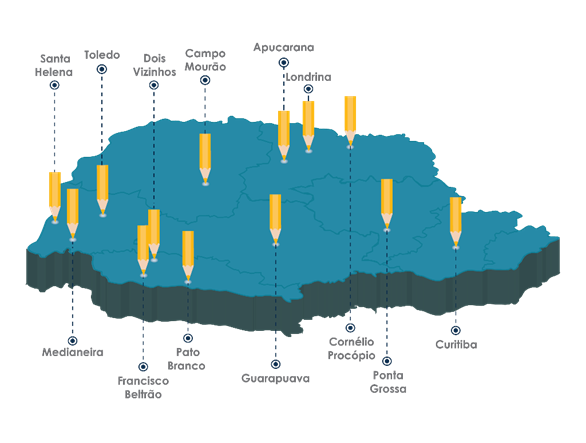
\includegraphics[width=0.7\textwidth]{Caps/Figs/campus_utfpr.png}
        \fonte{\utf}
        \label{fig:13campi}
    \end{figure}
    
    \begin{quadro}
        \centering
        \caption[Diferentes denominações da UTFPR]{As diferentes denominações da UTFPR ao longo de sua existência}        
        \label{qua:denomi}
		\begin{tabularx}{0.7\textwidth}{c >{\centering\arraybackslash}X}
			\toprule%
			\rowcolor{white}\bfseries Ano & \bfseries Denominação\\
			\midrule
			\csvreader[	head to column names,
						late after line=\csvifoddrow{\\}{\\\rowcolor{gray!10}}, 
						separator=pipe]%
						{Caps/Quadros/denominacoesUtfpr.csv}{}%
						{\ano & \denominacao}%
			\bottomrule
			\end{tabularx}
    \end{quadro}

\section{HISTÓRICO DO CÂMPUS}

O município de Toledo está situado na região Oeste do Paraná à 555 km de Curitiba e à 1445 km de Brasília. Pela sua localização geográfica, constitui uma área geopolítica estratégica e de relevância para a integração dos povos do Cone Sul da América. A cidade de Toledo possui aproximadamente 144 mil habitantes, conforme estimativa do Instituto Brasileiro de Geografia e Estatística (IBGE) \cite{ibge2020}.

\nomenclature[A]{IBGE}{Instituto Brasileiro de Geografia e Estatistica}

O município de Toledo é polo microrregional, sede da 18\textordfeminine{} Região Administrativa do Estado do Paraná, congregando 21 municípios que juntos totalizam mais de 350.000 habitantes. O desenvolvimento econômico do município tem atraído crescente número de jovens que buscam oportunidades de trabalho, de estudo e desenvolvimento cultural.

Em face ao projeto de expansão da rede pública federal de ensino, em 2006, a Prefeitura Municipal de Toledo, em conjunto com a Fundação Educacional de Toledo (FUNET) e com o apoio de parlamentares da região protocolou junto ao Governo Federal a solicitação de implantação do Campus Toledo. No mesmo ano realizou-se o exame de seleção para o curso Técnico Integrado em Gastronomia.

\nomenclature[A]{FUNET}{Fundação Educacional de Toledo}

Em 8 de janeiro de 2007 o campus Toledo deu início às suas atividades, sendo oficialmente inaugurado no dia 5 de fevereiro de 2007. Em 12 de fevereiro de 2007 iniciaram-se as aulas do curso Técnico Integrado em Gastronomia. Em agosto do mesmo ano, iniciaram-se as aulas do curso superior de Tecnologia em Processos Químicos no período noturno.

Em 2009 o curso Técnico Integrado em Gastronomia deu lugar ao Curso Técnico Integrado em Informática, o mesmo ano em que o curso superior de Engenharia Industrial Elétrica com ênfase em Automação iniciou suas atividades.

Em 2010 foi vez dos cursos de Engenharia Civil e Licenciatura em Matemática iniciarem suas atividades. Entretanto, nesse mesmo ano, em função das políticas internas da UTFPR, o curso Técnico Integrado em Informática teve sua última entrada de discentes.

Em 2013 o curso Técnico Integrado em Informática formou sua última turma e cedeu lugar para o curso superior de Tecnologia em Sistemas para Internet, o qual iniciou suas atividades no primeiro semestre de 2014. Ainda em 2014 o câmpus Toledo foi contemplado com a autorização para implantação de dois novos cursos de graduação. Assim, os cursos de Engenharia da Computação e Engenharia Bioprocessos e Biotecnologia iniciaram as suas atividades no primeiro semestre de 2015. Nesse mesmo ano foi aberto também o curso de pós-graduação em nível de mestrado acadêmico em Processos Químicos e Biotecnológicos. No ano de 2017, o campus Toledo obteve aprovação para abertura do curso de pós-graduação em nível de mestrado profissional em Matemática com ingresso de alunos previsto para início de 2018. Em 2019, também foi aprovado o Programa de Pós-Graduação em Tecnologias em Biociências (PPGBio) em nível de mestrado profissional.

\nomenclature[A]{PPGBio}{Programa de Pós-Graduação em Tecnologias em Biociências}

\section{HISTÓRICO DO DEPARTAMENTO E/OU DO CURSO}

O curso de graduação em Engenharia Eletrônica no campus Toledo teve o seu funcionamento aprovado pela Resolução N\textordmasculine{} 76/08 – COEPP de 15/08/2008. Iniciou suas atividades em 2009, localizado na Fundação Educacional de Toledo – FUNET, ainda com a denominação de curso de Engenharia Industrial Elétrica com Ênfase em Automação, buscando atender às necessidades da região de qualificação de profissionais atuantes no setor eletroeletrônico e de automação.

\nomenclature[A]{COEPP}{Conselho de Ensino Pesquisa e Pós-graduação da UTFPR}

Em julho 2009 o Ministério da Educação (MEC) publicou um novo catálogo de cursos, em que todas as Engenharias relacionadas a Elétrica deveriam se enquadrar em uma destas cinco categorias: elétrica, eletrônica, controle e automação, telecomunicações e computação. Em função deste catálogo, o colegiado do curso da época decidiu optar por Engenharia Eletrônica. Então, a partir do primeiro semestre de 2010, com mudanças efetuadas na matriz curricular para se enquadrar ao novo catálogo, o curso passou a ser ofertado à comunidade como Engenharia Eletrônica.

\nomenclature[A]{MEC}{Ministério da Educação}

No período de 2010 à 2011 ocorreu a construção e entrega dos Blocos A e C do campus Toledo e o curso foi transferido da FUNET para o campus. As salas de aula e laboratórios do curso foram instalados no Bloco A.

Em meados de 2012, o curso foi submetido ao processo de reconhecimento pelo MEC, obtendo conceito 4.

No ano de 2013, o quadro de professores em regime de dedicação exclusiva totalizava 12 profissionais e ocorreu a formatura da primeira turma do curso de graduação em Engenharia Eletrônica.

\subsection{Primeira atualização na matriz curricular}

Com cinco anos e meio de funcionamento, os professores do curso observaram que alguns ajustes na matriz curricular poderia melhorar  o desempenho dos discentes. Além disso, a alteração também foi motivada pela sinalização do Conselho Regional de Engenharia e Agronomia do Paraná (CREA-PR) que iria atualizar os critérios para concessão do artigo 8\textordmasculine{} da Resolução CONFEA 218/1973 (atribuição na modalidade de eletrotécnica) para os engenheiros recém formados. Até então, os alunos estavam recebendo essa atribuição, mas com as mudanças propostas pelo CREA-PR os novos alunos formados poderiam não obter o artigo 8\textordmasculine{}. Como a região Oeste do Paraná tem uma demanda considerável por Engenheiros Eletricistas, decidiu-se assegurar a aos discentes a garantia da atribuição na modalidade de eletrotécnica. Sendo assim, em 2015, o Núcleo Docente Estruturante (NDE) do curso iniciou discussões para alteração da matriz curricular. Ao final, foi redigido um documento com as modificações propostas que foi aprovado pelo Colegiado do curso e pelo Conselho de Graduações e Educação Profissional da UTFPR (COGEP) por meio da Resolução n\textordmasculine{} 067/15. De forma resumida as modificações aprovadas foram as seguintes:

\nomenclature[A]{CREA-PR}{Conselho Regional de Engenharia e Agronomia do Paraná}
\nomenclature[A]{CONFEA}{Conselho Federal de Engenharia e Agronomia}
\nomenclature[A]{NDE}{Núcleo Docente Estruturante}
\nomenclature[A]{COGEP}{Conselho de Graduações e Educação Profissional da UTFPR}

\begin{itemize}
	\item Deslocamento da disciplina de Física 3 do 2\textordmasculine{} período para o 3\textordmasculine{}  e alteração do pré-requisito;
	
	\item Deslocamento da disciplina de Física 4 do 3\textordmasculine{} período para o 5\textordmasculine{};
	
	\item Deslocamento da disciplina de Probabilidade e Estatística do 5\textordmasculine{} período para o 2\textordmasculine{} e alteração do pré-requisito;
	
	\item Substituição da disciplina de Fundamentos de Programação 2 (60 h) por Fundamentos de Programação Orientada à Objetos (60 h);
	
	\item Substituição da disciplina obrigatória de Instalações Industriais (90 h) pela optativa de Instalações Elétricas Industriais (60 h);
	
	\item Redução da carga horária das optativas de 300 horas para 180 horas;
	
	\item Substituição da disciplina de Fundamentos de Engenharia de Segurança do Trabalho (45 h) para a disciplina de Introdução à Engenharia de Segurança do Trabalho (30 h);
	
	\item Substituição da disciplina de Princípios de Comunicação (75 h) para a disciplina de Fundamentos de Sistemas de Comunicação (60 h);
	
	\item Substituição da disciplina de Circuitos Elétricos 3 (60 h) por Medidas e Sensores (45 h);
	
	\item Deslocamento da disciplina de Materiais e Equipamentos Elétricos do 3\textordmasculine{} período para o 5\textordmasculine{};
	
	\item Mudança da disciplina de Economia do 7\textordmasculine{} período para o 8\textordmasculine{};
	
	\item Alteração do pré-requisito da disciplina de Circuitos Elétricos 1 de Física 3 para Cálculo Diferencial e Integral;
	
	\item Substituição da disciplina de Instalações Prediais (90 h) por Instalações Elétricas Prediais (60 h);
	
	\item Substituir Máquinas Elétricas 1 (60 h) e Máquinas Elétricas 2 (60 h) pela disciplina de Conversão de Energia 1 (60 h);
	
	\item Substituir Máquinas Elétricas 3 (60 h) e Acionamentos Eletromagnéticos (60 h) pela disciplina de Máquinas e Acionamentos (60 h);
	
	\item Criação da disciplina optativa com o nome de Geração, Transmissão e Distribuição de Energia Elétrica (60 h) - alteração visa atender a carga horária mínima para obtenção do artigo 8\textordmasculine{} da Resolução CONFEA 218/1973 (atribuição na modalidade de eletrotécnica);
	
	\item Substituição da disciplina optativa de Sistemas de Potência 1 (75 h) pela optativa de Sistemas de Potência (60 h);
	
	\item Alteração do nome da disciplina de Fundamentos de Programação 1 (60 h) para Fundamentos de Programação (60 h);
	
	\item Deslocamento da disciplina de Metodologia de Pesquisa do 2\textordmasculine{} período para o 8\textordmasculine{};
	
	\item O pré-requisito do Trabalho de Conclusão de Curso 1 foi alterado para: Metodologia de Pesquisa e ter cursado o 7\textordmasculine{} período.
	
	
\end{itemize}

A nova matriz começou a vigorar em 2016 para todos os alunos.

\subsection{Segunda atualização na matriz curricular}

No primeiro semestre de 2018, o NDE do curso propôs a inclusão da disciplina de Eletrônica Analógica 1 como pré-requisito de Medidas e Sensores. Para desenvolver os conteúdos da ementa da disciplina de Medidas e Sensores é necessário um conhecimento básico sobre dispositivos semicondutores (diodos e transistores) – conteúdo abordados em Eletrônica Analógica 1. Sem o pré-requisito proposto seria necessário realizar uma atividade de nivelamento para poder introduzir alguns tópicos da ementa para alunos que ainda não haviam cursado Eletrônica Analógica 1. Por isso, o Colegiado do Curso resolveu aprovar a alteração proposta e enviá-la para apreciação pelo COGEP. Em 04 de junho de 2018 foi publicada a Resolução nº 36/2018 aprovando a alteração, a qual começou a vigorar a partir do segundo semestre de 2018. Maiores detalhes sobre essa alteração podem ser obtidos acessando ao processo SEI 23064.014304/2018-42.

\subsection{Terceira atualização na matriz curricular}

No segundo semestre de 2018, o NDE do curso propôs mais algumas alterações. Foi identificado que a disciplina de Comunicação Oral e Escrita poderia ser alterada para a disciplina de Comunicação Linguística, adotada pelos outros cursos do campus. Dessa forma haveria uma compatibilização das disciplinas entre cursos, maior flexibilização curricular para o aluno. Adicionalmente, a ementa de Comunicação Linguística está atualizada e dentro da formação pretendida. 

A disciplina de Cálculo Diferencial e Integral 3 no curso de Engenharia Eletrônica também tem ementa que não era compatível integralmente com os outros cursos de engenharia do campus. Por isso, resolveu-se adotar a ementa já utilizada nos cursos de Engenharia da Computação e Engenharia Civil. A única mudança foi na ementa da disciplina. Comparando o texto da ementa antiga com o texto da atual o conteúdo ``Funções de variável complexa'' foi excluído. O NDE considerou que esta exclusão não acarretaria problemas ao curso ao na formação dos alunos.

O NDE identificou disciplinas que normalmente apresentam altos índices de reprovação. Estas, poderiam ser divididas em duas, separando a parte teórica da prática. Com essa divisão o discente reprovado na parte teórica e aprovado na parte prática deixaria de consumir recursos do laboratório. Ademais, nas disciplinas iniciais a parte laboratorial fica bastante simples para o aluno reprovado, principalmente quando ele deixa para fazer a disciplina depois que já progrediu razoavelmente na matriz do curso. Dessa forma, o NDE propôs substituir a disciplina de Química, do segundo período, pelas disciplinas de ``Química Básica Teórica'' e ``Química Básica Experimental'' e substituir a disciplina de ``Circuitos Elétricos 1'' para ``Análise de Circuitos Elétricos 1'' e ``Laboratório de Circuitos Elétricos 1''.

O NDE também analisou a retirada de pré-requisito de 3 disciplinas: Probabilidade e Estatística, Empreendedorismo e Gestão de Projetos, aprovando a demanda.

\section{CONTEXTUALIZAÇÃO NACIONAL, REGIONAL E LOCAL}

O Engenheiro Eletrônico é um profissional extremamente flexível e imprescindível em muitos segmentos da economia, com atuação nas mais diferentes áreas da indústria, comércio especializado e serviço.

Nestes últimos anos, aconteceram muitas mudanças no cenário mundial; mudanças políticas, sociais e econômicas. Dessa forma, o estado do Paraná modificou sua política de desenvolvimento, saindo da atividade econômica voltada para a agricultura e pecuária, indo ao encontro da industrialização e consequente modernização de sua economia.

As novas tecnologias, com destaque para a eletrônica, estabeleceram uma nova organização e estrutura para a produção, do que decorre a necessidade de refletir e direcionar esforços para a formação de profissionais para o processo produtivo. Este novo cenário requer profissionais que possuam competências para projetar, executar e manter produtos e serviços que dinamizam o referido processo.

Dessa forma, a oferta do Curso de Engenharia Eletrônica, justifica-se pelos fatores elencados a seguir:

\begin{enumerate}
	
	\item O fato de a UTFPR consolidar-se cada vez mais como uma agência formadora de recursos humanos na área tecnológica;
	
	%\item Adequação do curso de Engenharia Elétrica, Ênfase em Automação, devido a recomendação do MEC para as Engenharias \pdfmarkupcomment{(MEC, 2009)}{não encontrei este documento}, às necessidades regionais;
	\item Adequação do curso de Engenharia Elétrica, Ênfase em Automação, atendendo às necessidades regionais;
	
	\item A oferta de um curso de engenharia visa contribuir com uma preocupação crescente: a carência de profissionais da área de engenharia eletrônica no Brasil;
	
	\item A região Oeste do Paraná possui potencial industrial comprovado, contando com parques industriais estruturados e indústrias nas áreas: alimentos, medicamentos, têxteis e metal mecânica. Além do potencial industrial, a região tem elevada produção agrícola, sendo seus expoentes a suinocultura, avicultura, produção de grãos e leitaria, o que possibilita que inúmeros dispositivos para automação e recursos informatizados possam ser projetados e disponibilizados visando a gestão mais eficiente destas produções.
	
\end{enumerate}


    
    % O TCC 1 deve conter:
    %   1 - Introdução
    %   2 - Objetivos
    %   3 - Justificativa
    %   4 - Referencial teórico
    %   5 - Materiais e métodos
    %   6 - Resultados esperados
    %   7 - Cronograma
    
    
    % Bibliografia
    \bibliography{references}
    
    \postextual
    
    % Apêndices:
    \apendices
    \chapter{Apêndice 1}
\label{apen:apen1}

\lipsum
    
    % Anexos:
    \anexos
    \chapter{Anexo 1}
\label{anex:anex1}

\lipsum
    
\end{document}
